\documentclass[a4paper,10pt]{article}

\usepackage[margin=1in]{geometry} 	% Setea el margen manualmente, todos iguales.
\usepackage[spanish]{babel} 		% {Con estos dos anda
\usepackage[utf8]{inputenc} 		% todo lo que es tildes y ñ}
\usepackage{fancyhdr} 			%{Estos dos son para
\usepackage{ulem}
\pagestyle{fancyplain} 			% el header copado}
\usepackage{color}			% Con esto puedo hacer la matufia de poner en color blanco un texto para engañar al formato
\usepackage{graphicx}	% Para insertar gráficos
\usepackage{array}			% Para usar arrays
\usepackage{hyperref}		% Para que tenga links el índice
\usepackage{lscape}         % Para apaisar figuras
\usepackage{ textcomp }
\usepackage{ulem}

%\usepackage{datetime}	% Para agregar automáticamente fecha/hora de compilación y otras cosas

\lhead{Bases de Datos} 	% {Con esto se usa el header copado. También está \chead para
\rhead{TP1} 	% el centro y comandos para el pie de página, buscar fancyhdr}
\renewcommand{\footrulewidth}{0.4pt}
\lfoot{Facultad de Ciencias Exactas y Naturales}
\rfoot{Universidad de Buenos Aires}
%\rfoot{\textit{}}
\usepackage{amsfonts}	% para simbolos de reales, naturales, etc. se usa \mathbb{•} y la letra
\usepackage{amsmath}	% para \implies
%\usepackage{algorithm}
%\usepackage{algorithmic}
\usepackage{caratula}
\usepackage{pdfpages}

%%%%%%%%%%%%%%%%%%%%%%%%%%%%%%%%%%%%%
%      COMANDOS ÚTILES USADOS       %
%%%%%%%%%%%%%%%%%%%%%%%%%%%%%%%%%%%%%

% \section{title} 		Te hace un título ``importante'' en negrita, numerado. También está \subsection{title} y \subsubsection{title}.
% \begin{itemize}		Te hace viñetas.
%	\item esto es un item	Cambiar itemize por enumerate te hace una numeración.
% \end{itemize}

% \textbf{text} 		Te hace el texto en negrita (bold).
% \underline{text}		Te subraya el texto.

% \textsuperscript{text}	Te hace ``superindices'' con texto. En teoría subscript debería funcionar, pero se puede usar guion bajo entre llaves
% 				y signos peso para hacerlo como alternativa. Sino buscar.

% \begin{tabular}{cols} 	Es para hacer tablas. Se pone una c por cada columna deseada dentro de cols (si es que se desea centrada, l para justificar a 
%	a & b & c		izquierda, r a la derecha). Si se separa por espacios la tabla no tendrá líneas divisorias. Si se separa por | en lugar de 
% \end{tabular}			espacios, aparecerá una línea. Con || dos, y así. Luego para los elementos de las filas se escriben y se separan con ampersand (&).
%				Finalmente, para las líneas horizontales, se usa \hline para una linea en toda la tabla y \cline{i - j} te hace la linea desde
%				la celda i hasta la j, arrancando en 1.
%				Si en la columna se pone p(width) podés escribir un párrafo en la celda. Para hacer un enter con \\ no funciona porque te hace un
%				enter en la fila. Para eso se usa el comando \newline.
  
% \textcolor{color predefinido en palabras}{text}

%%%%%%%%%%%%%%%%%%%%%%%%%%%%%%%%%%%%%
%    FIN COMANDOS ÚTILES USADOS     %
%%%%%%%%%%%%%%%%%%%%%%%%%%%%%%%%%%%%%

\newcommand{\Gather}[1]{\begin{gather*}#1\end{gather*}}
%\newcommand{\Def}[1]{\textbf{Definición: }#1}
%\newcommand{\Prop}[1]{\textbf{Propiedad: }#1}
%\newcommand{\Teo}[1]{\textbf{Teorema: }#1}
\newcommand{\Obs}[1]{\textbf{Observación: }#1}
%\newcommand{\Amat}{A \in \mathbb{R}^{n\textnormal{x}n}}
\newcommand{\filtro}[1]{\textbf{\textit{#1}}}
\renewcommand{\labelenumii}{\theenumii}
\renewcommand{\theenumii}{\theenumi.\arabic{enumii}.}

\begin{document}

%%%%%%%%%%%%%%%%%%%%%%%%%%%
%			INICIO DE CARÁTULA			%
%%%%%%%%%%%%%%%%%%%%%%%%%%%

%% **************************************************************************
%
%  Package 'caratula', version 0.2 (para componer caratulas de TPs del DC).
%
%  En caso de dudas, problemas o sugerencias sobre este package escribir a
%  Nico Rosner (nrosner arroba dc.uba.ar).
%
% **************************************************************************



% ----- Informacion sobre el package para el sistema -----------------------

\NeedsTeXFormat{LaTeX2e}
\ProvidesPackage{caratula}[2003/4/13 v0.1 Para componer caratulas de TPs del DC]


% ----- Imprimir un mensajito al procesar un .tex que use este package -----

\typeout{Cargando package 'caratula' v0.2 (21/4/2003)}


% ----- Algunas variables --------------------------------------------------

\let\Materia\relax
\let\Submateria\relax
\let\Titulo\relax
\let\Subtitulo\relax
\let\Grupo\relax


% ----- Comandos para que el usuario defina las variables ------------------

\def\materia#1{\def\Materia{#1}}
\def\submateria#1{\def\Submateria{#1}}
\def\titulo#1{\def\Titulo{#1}}
\def\subtitulo#1{\def\Subtitulo{#1}}
\def\grupo#1{\def\Grupo{#1}}


% ----- Token list para los integrantes ------------------------------------

\newtoks\intlist\intlist={}


% ----- Comando para que el usuario agregue integrantes

\def\integrante#1#2#3{\intlist=\expandafter{\the\intlist
	\rule{0pt}{1.2em}#1&#2&\tt #3\\[0.2em]}}


% ----- Macro para generar la tabla de integrantes -------------------------

\def\tablaints{%
	\begin{tabular}{|l@{\hspace{4ex}}c@{\hspace{4ex}}l|}
		\hline
		\rule{0pt}{1.2em}Integrante & LU & Correo electr\'onico\\[0.2em]
		\hline
		\the\intlist
		\hline
	\end{tabular}}


% ----- Codigo para manejo de errores --------------------------------------

\def\se{\let\ifsetuperror\iftrue}
\def\ifsetuperror{%
	\let\ifsetuperror\iffalse
	\ifx\Materia\relax\se\errhelp={Te olvidaste de proveer una \materia{}.}\fi
	\ifx\Titulo\relax\se\errhelp={Te olvidaste de proveer un \titulo{}.}\fi
	\edef\mlist{\the\intlist}\ifx\mlist\empty\se%
	\errhelp={Tenes que proveer al menos un \integrante{nombre}{lu}{email}.}\fi
	\expandafter\ifsetuperror}


% ----- Reemplazamos el comando \maketitle de LaTeX con el nuestro ---------

\def\maketitle{%
	\ifsetuperror\errmessage{Faltan datos de la caratula! Ingresar 'h' para mas informacion.}\fi
	\thispagestyle{empty}
	\begin{center}
	\vspace*{\stretch{2}}
	{\LARGE\textbf{\Materia}}\\[1em]
	\ifx\Submateria\relax\else{\Large \Submateria}\\[0.5em]\fi
	\par\vspace{\stretch{1}}
	{\large Departamento de Computaci\'on}\\[0.5em]
	{\large Facultad de Ciencias Exactas y Naturales}\\[0.5em]
	{\large Universidad de Buenos Aires}
	\par\vspace{\stretch{3}}
	{\Large \textbf{\Titulo}}\\[0.8em]
	{\Large \Subtitulo}
	\par\vspace{\stretch{3}}
	\ifx\Grupo\relax\else\textbf{\Grupo}\par\bigskip\fi
	\tablaints
	\end{center}
	\vspace*{\stretch{3}}
	\newpage}

\materia{Bases de Datos}
\submateria{Segundo Cuatrimestre de 2014}
\titulo{Trabajo Práctico 2 - Estimadores}

\grupo{}
\integrante{Martinez Suñe, Agustín}{630/11}{aemartinez@dc.uba.ar}
\integrante{Iglesias, Axel}{79/10}{axeligl@gmail.com}
\integrante{Lascano, Nahuel}{476/11}{laski.nahuel@gmail.com}
\integrante{Artuso, Pablo}{282/11}{artusopablo@gmail.com}

\begin{titlepage}
\maketitle
\thispagestyle{empty}
\end{titlepage} 

%%%%%%%%%%%%%%%%%%%%%%%%%%%
%				FIN DE CARÁTULA			%
%%%%%%%%%%%%%%%%%%%%%%%%%%%

\tableofcontents
%\clearpage

%%%%%%%%%%%%%%%%%%%%%%%%%%%
%					DESARROLLO				%
%%%%%%%%%%%%%%%%%%%%%%%%%%%

\section{Introducción}
Con el avance de la tecnología y la capacidad de almacenamiento, las bases de datos tienden a almacenar cada vez más información. En un principio parece una ventaja, sin embargo, se puede inferir fácilmente que un almacenamiento masivo puede ocasionar problemas a la hora de realizar búsquedas. Mientras más grande es el espacio de búsqueda, mayor será el tiempo a invertir para lograr el objetivo.

El \textbf{optimizador de consultas}, componente clave del motor de base de datos, es el que combate el problema del tiempo antes mencionado. Su misión es, como bien explica su propio nombre, tratar de optimizar la forma de realizar la consulta con el fin de obtener la respuesta lo más rápido posible. Entre muchas otras cosas, el componente hace un fuerte uso de \textbf{estimadores} para poder llevar a cabo la optimización. Un \textbf{estimador} es un componente que brinda información aproximada de la cantidad de elementos que cumplen cierta condición (también llamada \textbf{selectividad}) comparativa contra una constante dada. Por lo tanto, el optimizador intentará reescribir la consulta de distintas maneras (manteniendo su valor semántico) y a través de distintas estimaciones, tomar una desición de cuál será la forma más eficiente de realizar la consulta. Si bien la precisión de la estimación debe ser lo más ajustada posible tiene también importancia la velocidad con la que se realiza, dado que este procedimiento se repetirá por cada consulta a la base. Es por esto que el estimador debe estar organizado de modo tal que pueda resolver rápidamente las consultas pedidas, quizás a cambio de tomarse más tiempo a la hora de inicializarlo o reiniciarlo. Del mismo modo, la elección del estimador afecta fuertemente la precisión de los resultados, por lo cual el conocimiento sobre la información específica de los elementos (distribución, dispersión, densidad, etc.) juega un papel determinante a la hora de la elección del estimador.

En el presente trabajo, detallamos tres implementaciones distintas de estimadores, mostrando sus diferentes comportamientos frente a distintas distribuciones, comparándolos y extrayendo conclusiones.
\section{Estimadores}
Los estimadores que diseñamos fueron tres: un estimador basado en histogramas clásicos (punto 4.1 del paper de Piatetsky-Shapiro), un estimador basado en ``pasos de distribución'' (punto 4.2 del mismo paper) y uno propio, diseñado a partir de observar un tipo de distribución en la cual los dos anteriores no funcionaban bien.

Los tres estimadores comparten una serie de premisas:
\begin{itemize}
 \item Reciben por parámetro una columna para hacer su estimación
 \item Reciben un parámetro extra que influye en algún aspecto de su comportamiento (en adelante llamado $S$)
 \item En su construcción pueden tomarse el tiempo que sea necesario para incializar sus estructuras...
 \item ...pero no pueden asumir que la columna completa entre en memoria. Es decir, deben hacer uso del motor de bases de datos para resolver las consultas que necesiten. 
 \item Una vez inicializados, deben responder rápidamente ambas consultas posibles: por igualdad (la probabilidad de que un elemento al azar de la columna sea igual a un $x_0$ pasado por parámetro) y por mayor (idem con mayor estricto en lugar de igual). Las llamamos $Sel(=x)$ y $Sel(>x)$.
\end{itemize}

Para realizar los análisis desde el punto de vista general y no entrar en casos borde poco probables, vamos a tomar como regla general que $S$ es ``pequeño'' respecto de la longitud del rango de la distribución\footnote{Llamamos $rango$ a la lista de enteros entre el elemento máximo y el mínimo de la distribución, es decir, a los valores que, asumimos, puede tomar un elemento de la distribución} (al menos un órden de magnitud menor).


\subsection{Estimador basado en Historgramas Clásicos}
La idea del estimador consiste en generar un histograma de la distribución para realizar las consultas rápidamente. El histograma generado tiene $S$ barras de ancho constante (el suficiente para cubrir toda la distribución) y altura variable dependiendo de la cantidad de elementos de la columna que ``caigan'' en el bucket. Notar que esto genera buckets con límites siempre distintos, pues son generados por una división regular del rango de la distribución.

Una vez construido el histograma, el estimador arma un histograma secundario ``normalizado'' cuyos límites coinciden con el principal pero cuyas barras fueron divididas por la cantidad de registros totales. A la hora de responder consultas usará este histograma, pues es más útil el porcentaje de elementos que caen en cada bucket que la cantidad absoluta.

Como el paper no especifica qué devolver a la hora de resolver las consultas por igualdad, analizamos dos opciones: está claro que el primer paso siempre es buscar el bucket correspondiente a $x_0$ (solo puede haber uno\footnote{Si es que lo hay. Si no lo hay, el estimador devuelve 0 pues ningún elemento puede ser igual a uno que cae fuera de la distribución.}) y obtener el valor correspondiente en el histograma de porcentajes. Ahora bien, podíamos elegir devolverlo directamente, con lo cuál en realidad estaríamos devolviendo la probabilidad de que un elemento caiga en el mismo bucket que $x_0$, o podemos dividir ese resultado por la longitud del bucket, dando algo más aproximado a una probabilidad de igualdad al elemento en sí. Inicialmente preferimos la primera opción, considerando que con la segunda estábamos asumiendo que la distribución (dentro del bucket) era uniforme y nos parecía una asunción demasiado fuerte. Pero pronto nos dimos cuenta de que la segunda tenía mucha mejor performance no solo en una distribución uniforme sino en todas, con lo cual decidimos quedarnos con esa\footnote{Por falta de tiempo y por no estar dentro de la consigna del trabajo no incluímos aquí dichos análisis, pero nos pareció una decisión relevante como para comentarla en esta sección.}. Analíticamente tiene sentido también, la probabilidad de un elemento no es la probabilidad del rango en el que cae sino que casi siempre suele ser menor.

A la hora de responder consultas por mayor el paper es más específico: hace falta responder un promedio entre la probabilidad de que un elemento caiga en un bucket mayor al de $x_0$ (la cual se obtiene sumando los porcentajes de todos los buckets mayores) y la probabilidad de que un elemento caiga en el mismo bucket que $x_0$ o en uno mayor (la cual se obtiene también sumando los porcentajes de ese bucket y los de todos sus buckets mayores). Es decir, la probabilidad termina siendo la suma entre
\begin{itemize}
 \item el porcentaje de elementos que caen en buckets mayores y
 \item la mitad del porcentaje correspondiente al bucket de $x_0$.
\end{itemize}
Es decir, a grandes rasgos se asume que $x_0$ tiene aproximadamente la mitad de los elementos de su propio bucket mayores que él. Esto puede parecer sensato en el caso general (pues intenta minimizar el error), el problema ocurre cuando $x_0$ comparte buckets con muchos elementos (lo cual puede pasar para distribuciones de rangos amplios pero muy concentradas en cierta región). En ese caso el porcentaje correspondiente al bucket de $x_0$ es grande, y el error por lo tanto también lo es\footnote{Intuitivamente, cuanto más lejos esté $x_0$ del ``centro'' del bucket, más diferencia habrá entre la probabilidad real y la estimada. Como esta diferencia solo está acotada por la mitad del porcentaje del bucket, un bucket con gran porcentaje puede producir un error inaceptable}. Este error, en casos exagerados, podría llegar a ser tan grosero como 50\% (el cual es alcanzable simplemente respondiendo siempre $0.5$), con lo cual el paper se propone buscar otro método de estimación que evite ese problema.

\subsection{Estimador basado en Distribution Steps}
Este estimador se propone alterar la idea del Histograma Clásico para atacar el problema recién mencionado. Lo resuelve armando un histograma donde todas las barras tienen siempre la misma altura, con lo cual evita el caso de un tener uno o pocos buckets con un gran porcentaje de la distribución concentrada en ellos, y permitiendo que varíe el ancho de las mismas. Esto trae aparejado un aumento en la complejidad de construcción y algoritmos no tan simples para resolver consultas, pues ahora hay que tener en cuenta los casos en que $x_0$, por ejemplo, coincide con el límite de varios buckets (lo cual en puede ocurrir para las distribuciones con muchos elementos similares).

La construcción nuevamente usa $S$ como la cantidad de buckets, intenta mantener invariante su altura y va eligiendo $S+1$ ``límites'' (llamados $bordes$ en nuestro código) elementos de la distribución, intentando mantener el invariante de que a la izquierda del límite $i$ haya un $(i*\frac{100}{S})\%$ de los elementos. Así, por ejemplo, para $S=10$ el límite 0 es el mínimo de la distribución, el límite $3$ tiene un $30\%$ de elementos a su izquierda, el 8 un $80\%$ y el 10 tiene todos los elementos a su izquierda (es el máximo de la distribución). Para esto es necesario ordenar primero los datos, lo cual implica un costo mayor que en el Histograma Clásico que solo necesita hacer recorridas lineales para buscar máximo y mínimo y luego para ubicar cada elemento en su bucket.

El paper presenta dos opciones distintas para resolver las consultas de este algoritmo una vez generado el estimador: una que minimiza el error en el peor caso y otra que lo minimiza en el caso promedio (pero tiene un error un mayor en el peor caso). Según argumenta, este último suele funcionar mejor en distribuciones de la vida real y específicamente para su utilización en optimización de consultas, por lo que elegimos implementar la versión que minimiza el error en el caso promedio.

Para ese método, el paper utiliza (y da un algoritmo para calcular) un valor llamado $densidad$ de la distribución: un número entre 0 y 1 que intuitivamente intenta aproximar el porcentaje promedio de valores iguales entre sí\footnote{Por ejemplo, una distribución con un solo valor tendrá densidad 1, una con todos valores distintos tendrá densidad $\frac{1}{\#elementos}$.}. Luego, define $\delta = min(\frac{0.5}{S}, densidad)$\footnote{Un análisis simple revela que en buena parte de los casos $\delta = densidad$, pues para que no lo fuese tendría que pasar $\frac{0.5}{S} < densidad$, es decir $0.5 < densidad*S$ (pues $S$ es siempre $>0$). Para visualizar lo fuerte de la implicación, tomemos por ejemplo un $S=100$ (relativamente grande) y una distribución de rango $10000$: para alcanzar la densidad necesaria debería tomar solo 50 valores distintos. Naturalmente puede ocurrir, pero son distribuciones particulares de las que hablaremos más adelante y no el caso general. Como además asumimos que $S$ es comparativamente pequeño respecto del rango, es seguro suponer para los análisis teóricos que efectivamente $\delta = densidad$.}.

Como la altura de los buckets no aporta información en este estimador (siempre es la misma) sus algoritmos se basan mayormente en saber en qué bucket cae el estimador (para la selectividad por mayor), en si coincide o no con uno o varios límites entre buckets y si esos límites incluyen o no extremos, y en el valor de $\delta$. Un detalle a destacar es que para los casos en el que $x_0$ coincide con dos o más límites entre buckets (sean estos extremos o no) el paper recurre a las versiones del algoritmo que minimizan el error en el peor caso (sin dar mucha explicación del motivo). Es por esto que en esos casos el algoritmo no usa el valor de $\delta$ (que se introduce solo en la sección donde se explica cómo minimizar el error promedio). En general las fórmulas que utiliza el estimador están pobremente fundamentadas, diciendo únicamente que ``En la práctica se demostraron muy precisas, incluso más que las anteriores [las que minimizan el error en el peor caso]''.

Para resolver consultas por igualdad, el estimador usa fuertemente el valor de $\delta$. Averiguar en qué bucket cae $x_0$ carece de utilidad en este caso, pues la altura de los mismos no aporta información y tampoco su distancia a los extremos. Sí importa separar los casos en los que coincide con el límite de varios buckets y/o con el de los extremos. Según el caso, el estimador devolverá directamente $\delta$ (si $x_0$ coincide con ningún o un límite no-extremo) o $\frac{\delta}{2}$ (si coincide con el máximo o el mínimo). En los casos en los que $x_0$ coincide con dos o más límites, devolverá $\frac{K}{S}$ (donde $K$ es la cantidad de límites con los cuales coincide) en caso de que ninguno sea extremo, o $\frac{K-0.5}{S}$ en caso de que alguno sea el mínimo o el máximo. Restan dos casos borde:
\begin{itemize}
 \item Si el valor coincide tanto con el mínimo como con el máximo entonces todos los elementos de la distribución son iguales a $x_0$, con lo cual la probabilidad es 1.
 \item Si el valor es menor al mínimo o mayor al máximo está fuera de la distribución, con lo cual la probabilidad es 0.
\end{itemize}

Para las consultas por mayor, el estimador recurrre a las fórmulas definidas en el paper pero considerando que estas en realidad sirven para calcular la selectividad por menor, con lo cual debe utilizar $Sel(>x_0) = 1 - Sel(<x_0) - Sel(=x_0)$\footnote{Lo cual vale por los axiomas definidos en el paper, en particular $Consistency$.}. Dichas fórmulas son (llamando $X$ al índice del bucket más a la izquierda que incluya valores iguales a $x_0$ y $K$ a la cantidad de límites con los que $x_0$ coincida):
\begin{itemize}
 \item si $x_0$ no coincide con ningún límite, $\frac{X+0.5}{S} - \frac{\delta}{2}$
 \item si $x_0$ coincide con un límite no-extremo, $\frac{X}{S} - \frac{\delta}{2}$
 \item si $x_0$ coincide con varios límites no-extremos, $\frac{X-0.5}{S}$
 \item si $x_0$ coincide con varios límites incluyendo el máximo, $1 - \frac{K-0.5}{S}$
 \item si $x_0$ coincide solo con el máximo, $1 - \frac{\delta}{2}$
\end{itemize}
y por último, dos casos borde:
\begin{itemize}
 \item si $x_0$ coincide con el mínimo o es menor, $0$
 \item si $x_0$ es mayor que el máximo, $1$
\end{itemize}

\subsection{Estimador Propio}
Al realizar los análisis de los estimadores presentados en el paper, descubrimos un caso en el cual ninguno de los dos es muy preciso: cuando el rango es grande pero los elementos toman pocos valores dentro de él (llamamos a estas \textbf{distribuciones esparsas}) con lo que nos propusimos encontrar un estimador que los resuelva correctamente. Fue así que dimos con el estimador CuentaApariciones\texttrademark que resuelve estos casos a la perfección. A la hora de su creación, genera dos diccionarios:
\begin{itemize}
 \item El primero guarda, para cada elemento, su cantidad de apariciones en la columna.
 \item El segundo guarda, para cada elemento, la suma de su cantidad de apariciones y las de todo elemento menor (como el anterior pero con el acumulado hasta el momento).
\end{itemize}

Luego, para resolver las consultas por igualdad simplemente tiene que devolver la cantidad de apariciones del elemento (que puede ser 0 si no está en los diccionarios) sobre la cantidad de elementos totales, y esto lo puede computar fácilmente buscando $x_0$ en el primer diccionario.

Para resolver las consultas por mayor hay tres casos:
\begin{itemize}
 \item Si el elemento aparece en la distribución solo tiene que calcular el porcentaje de elementos mayores a él, esto es, $\frac{T-acum(x_0)}{T}$ con $T$ = la cantidad total de elementos y $acum(x_0)$ = el acumulado del elemento $x_0$.
 \item Si el elemento no aparece en la distribución pero cae dentro ($min < x_0 < max$) también hay que calcular el porcentaje de elementos mayores a él, lo cual se logra computando $Sel(>menor_inmediato(x_0))$ donde $menor_inmediato(x_0)$ es el máximo elemento menor a $x_0$ que sí aparece en la distribución.
 \item Si el elemento cae fuera de la distribución, procedemos como de costumbre devolviendo $1$ si es $<min$ o $0$ si es $>max$.
\end{itemize}
Esto se calcula rápido si el elemento está en la distribución (solo hay que buscarlo en el segundo diccionario) o está fuera del rango, y un poco más lento si está dentro del rango pero no aparece (porque hay que buscar en los diccionarios el máximo elemento menor que sí aparezca).

Para aprovechar el parámetro de algún modo, decidimos hacer un caché con los $S$ elementos más frecuentes, y armar un diccionario específico para ellos que es el primero en ser consultado. La precisión del algoritmo no depende del parámetro pero sí su velocidad.

Notar que el primer diccionario es equivalente a un histograma donde todos los buckets tienen ancho 1 (aunque optimizado en su consumo de memoria para no guardar los elementos que no aparecen). Relacionado con esto, debemos aclarar que este estimador asume fuertemente que la cantidad de elementos distintos de la distribución entra en la memoria, pues guarda para cada uno de ellos dos enteros con información. Si se lo usa con distribuciones extensas y densas, su consumo de memoria es mucho mayor al de los otros estimadores.
\section{Análisis teórico}
En esta sección realizamos un análsis teórico sobre la performance de los tres estimadores para tipos de distribuciones variados.

Compararemos primero los dos estimadores sugeridos por la materia y luego haremos un apartado especial para el nuestro.

\subsection{Performance en distribuciones uniformes}
Para responder la pregunta de qué estimador debe exhibir mejor performance en un dataset con distribución uniforme, hace falta primero analizar con detenimiento este tipo de distribución. La distribución uniforme ``reparte'' los elementos en el rango disponible de forma equitativa: todos los enteros tienen la misma probabilidad de ocurrir.

Es decir, la forma de un Histograma Clásico de la distribución tendrá todas las barras del mismo ancho (por invariante de construcción del histograma) y de la misma altura, pues todos los rangos de idéntico ancho tienen aproximadamente la misma cantidad de elementos.

A su vez, la forma de un histograma de Distribution Steps tendrá todas las barras de la misma altura (por invariante de construcción del histograma) y del mismo ancho, pues la cantidad de elementos que resulta ser menor a un cierto porcentaje de los demás está relacionado directamente con ese porcentaje. Dicho en otras palabras, suponiendo un histograma de 10 barras, estas tendrán un ancho aproximado al 10\% del rango de la distribución, pues eso mantiene la condición (propia de Distribution Steps) de que el límite i deja a su izquierda $10i\%$ de los elementos (ver la sección de Estimadores para más información).

Entonces concluimos que dado un mismo parámetro $S$ ambas distribuciones ``dibujarán'' prácticamente el mismo histograma. Esto podría inducir a pensar que la respuesta podría ser similar y que por lo tanto la performance será la misma, pero estaríamos olvidando que ``usan'' esos histogramas de maneras distintas.


\subsubsection{Consultas por igualdad}
Para las consultas por igualdad el Histograma Clásico computa la probabilidad dividiendo la altura de la barra en la que cae $x_0$ por la cantidad de elementos totales ($T$), y dividiendo nuevamente por el ancho de la barra ($~T/S$). De este modo, por ejemplo, si $S$ es 20 y el rango es 1000, una distribución uniforme producirá una respuesta aproximada a $\frac{\frac{50}{1000}}{50} = 0,1\%$ (pues todas las barras tendrán altura aproximada = 50), la cual es una excelente estimación para cualquier $x_0$ en una distribución uniforme (porque coincide con la esperanza de su porcentaje de apariciones). Y podemos ver que esta estimación no depende de $S$, pues $T/S$ aparece tanto como producto como divisor con lo cual se cancelan. Concluimos entonces que la performance del Histograma Clásico no dependerá del parámetro, y que su performance por igualdad será muy buena en una distribución uniforme.

Por otro lado, el método de Distribution Steps (en su versión que minimiza el error en el caso promedio, que es la elegimos implementar) computa en el momento de su construcción el $\delta$ del que ya hablamos y responde basándose en ese valor. En particular en el caso más probable para una distribución uniforme (que $x_0$ coincida con a lo sumo un límite entre buckets, y no con uno extremo\footnote{Este caso es el más probable pues difícilmente en una distribución uniforme coincidan en valor varios límites de buckets: significaría que hay más elementos de ese valor de los que entran en dos buckets, pero para cantidades pequeñas de $S$ en relación al rango de la distribución es muy difícil que ocurra}) el estimador responde exactamente ese $\delta$. Es decir, antes que nada, que su performance difícilmente dependa de $S$ (la cantidad de buckets) salvo que sea tan grande (en relación al rango de la distribución) como para que muchos elementos del mismo valor se extiendan a lo largo de varios buckets. Veamos entonces si ese $\delta$ es una buena estimación en el caso de una distribución uniforme.

$\delta$ es el mínimo entre $0.5/S$ y la densidad. Como ya dijimos, para valores razonables (no muy grandes) de $S$ y distribuciones densas (como es la uniforme) es muy probable que la densidad sea menor a $0.5/S$, por lo cual en general caeremos en el caso $\delta =  densidad$. Como la densidad, informalmente hablando, aproxima el porcentaje medio de valores iguales, en el caso de una distribución uniforme será muy cercana a $1$ sobre la cantidad de elementos distintos, lo cual es exactamente la probabilidad de que un elemento de una distribución uniforme sea igual a un $x_0$ cualquiera. Por esto concluimos que independientemente del parámetro elegido, Distribution Steps tendrá también buena performance por igualdad en una distribución uniforme.

\subsubsection{Consultas por mayor}
Recordemos que para las consultas por mayor el Histograma Clásico computa la selectividad haciendo el promedio entre la probabilidad de que un elemento caiga en buckets mayores al $x_0$ y la de que un elemento caiga en buckets mayores o en el mismo. Como ya comentamos, esto puede traer un error grande para distribuciones en las que los elementos están muy concentrados en pocas regiones. Pero este no es el caso de las distribuciones uniformes, por lo que suponemos que el estimador se comportará correctamente en líneas generales.

Por su lado, el método de Distribution Steps presenta comportamientos matemáticamente más complejos. Como su selectividad por mayor se basa en su selectividad por menor (además de su selectividad por igual, que ya fue analizada), nos resta analizar el error en $Sel(<x_0)$ para obtener una estimación del error total de $Sel(>x_0)$. Nuevamente podemos asumir que $x_0$ coincidirá a lo sumo con un límite no-extremo en la gran mayoría de los casos, con lo cual reducimos los casos interesantes a dos:
\begin{itemize}
 \item Si coincide con un límite no-extremo, $\frac{X}{S} - \frac{\delta}{2}$ será la respuesta. $\frac{X}{S}$ es el porcentaje de elementos a la izquierda de $x_0$, y $\frac{\delta}{2}$ es la mitad de $Sel(=x_0)$ en este mismo caso. Con esa resta entendemos que el algoritmo intenta considerar los casos en que hay más elementos iguales a $x_0$ a la izquierda del límite $X$, y asume que la mitad de ellos están a la izquierda (y la otra mitad a la derecha). La suposición es válida dentro del contexto de una distribución uniforme, con lo cual podemos suponer que la performance será buena.
 \item Si no coincide con ningún límite, $\frac{X+0.5}{S} - \frac{\delta}{2}$ será la respuesta. El razonamiento es similar, solo ``corremos'' el límite $X$ a la derecha $0.5$ asumiendo que $x_0$ cae aproximadamente en la mitad de su bucket. Nuevamente la suposición parece sensata en una distribución uniforme, con lo que asumimos que la performance estará bien.
\end{itemize}

Por último, hace falta aclarar que en ambos estimadores un mayor parámetro $S$ permitirá una precisión mayor, pues aumenta la ``definición'' de los buckets y con eso la veracidad de las suposiciones en las que se basan los estimadores. Como ambos asumen en algún momento que $x_0$ cae en la mitad de su bucket, cuantos menos elementos haya en los mismos más verdadera será la afirmación y por ende mejor será la performance. Concluimos entonces que a un mayor $S$ la performance de ambos estimadores mejorará.

\subsection{Performance en distribuciones normales}
La distribución normal presenta mucha concentración de datos alrededor de una media y va disminuyendo alrededor de ella.

\subsubsection{Consultas por igualdad}
El Histograma Clásico, asumiendo suficiente cantidad de buckets, podrá hacer estimaciones bastante cercanas a la realidad. Mejorará mucho a medida que $S$ aumente, porque podrá evaluar más precisamente las diferentes secciones 


\subsection{Performance de nuestro estimador propio}
Dado que nuestro estimador obtiene el histograma más detallado posible de la distribución que analiza (pues todo bucket tiene ancho 1) podemos decir que no pierde información. A partir de una instancia de nuestro estimador se puede reconstruir la distribución entera, con lo cual CuentaApariciones\texttrademark es \textbf{perfecto}. Su error siempre será 0 porque tiene en él toda la información necesaria. ¿Dónde está el truco?

Los problemas son tres:
\begin{itemize}
 \item A decir verdad, sí pierde información: se pierde el orden en el que estaban los datos. No se puede reconstruir la columna, solo su multiconjunto de elementos.
 \item Ocupa grandes cantidades de memoria en el caso general. Para darnos una idea, en una distribución de rango un millón con todos los valores poblados, el estimador consume alrededor de 8MB. Puede parecer poco, pero si consideramos que en general las bases de datos usan estimadores para todos los atributos numéricos y en tablas variadas, el número puede salirse de control bastante rápidamente.
 \item Puede ponerse lento para calcular $Sel(>x_0)$ si $x_0$ no aparece en la columna. Tarda tiempo lineal en la cantidad de valores distintos de los elementos (porque hace una búsqueda lineal del máximo elemento menor a $x_0$), lo cual puede ser demasiado tiempo para una gran cantidad de valores distintos.
\end{itemize}

Entonces, concluimos que es un excelente estimador para distribuciones esparsas o de rangos pequeños, pero que puede no funcionar bien para distribuciones densas y muy extensas, y no escala para varias columnas en varias tablas. Lo cual nos lleva a la proxima sección...

\subsection{Distribuciones en las que los estimadores exhiben baja perfomance}
Mencionamos ya un poco este tema en la sección de estimadores. Miremos primero la selectividad por igualdad.
\begin{itemize}
 \item El estimador por Histogramas Clásicos presentará mala performance en una distribución con elementos distribuidos en intervalos y en el medio ``lagunas'' despobladas, por ejemplo la capacidad en GB de un conjunto de discos rígidos. Si la longitud de las lagunas es menor que el ancho de los buckets, siempre que sea consultado por elementos que caigan en las ``lagunas'' responderá una probabilidad grande cuando en realidad la respuesta correcta será 0. Si el ancho de los buckets es menor al de las lagunas, de todos modos la performance será mala en los valores cercanos a los que sí aparecen en la distribución.
 \item El estimador de Distribution Steps presentará mala performance en una distribución donde la simple densidad no sea un buen representante de la probabilidad. Por ejemplo, con elementos distribuidos de formas poco equitativas, donde algunos valores tengan muchos representantes y otros pocos.
\end{itemize}
Respecto a la selectividad por mayor:
\begin{itemize}
 \item Como ya mencionamos, el estimador de Histogramas Clásicos funcionará mal en distribuciones con muchos valores concentrados entre sí. Para valores pequeños de $S$, su estimación para valores que caigan en los buckets más poblados tiene un error muy grande.
 \item Nuevamente en una distribución con mucha variabilidad en sus datos, Distribution Steps se comportará pobremente a la hora de calcular $Sel(>x_0)$.
\end{itemize}
Repetimos que nuestro estimador es perfecto a nivel performance, sus problemas pasan por otro lado.
\section{Análisis empírico}

\subsection{Performance para distribuciones uniforme}
A continuación mostraremos cómo se comportaron los distintos estimadores en cuanto al error medio obtenido ante la variación del parámetro $S$ (llamado $p$ en el código) de entrada del estimador en una distribución uniforme. Para cada $S$ fueron realizadas $100$ consultas por igualdad y $100$ consultas por mayor.

La distribución uniforme utilizada tiene 10000 elementos de 1 a 10000.


\begin{figure}[h!]  
  \centering
  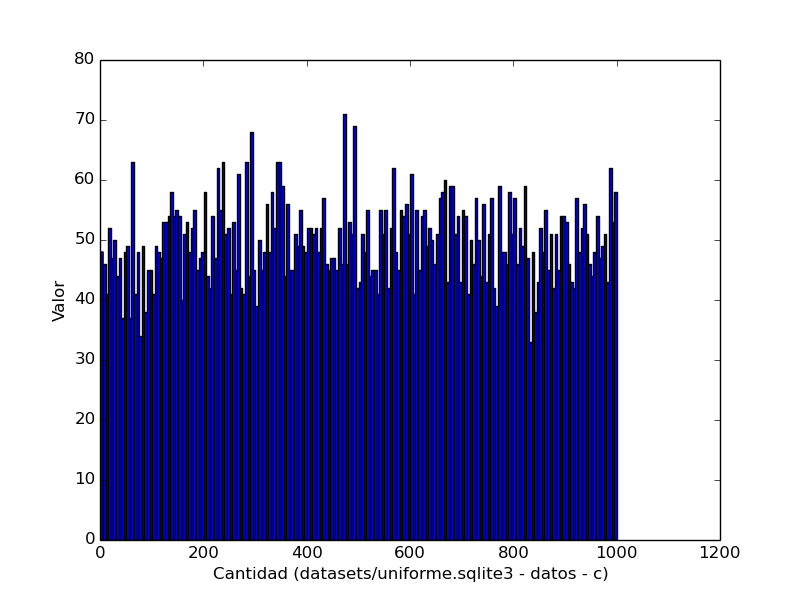
\includegraphics[width=0.45\textwidth]{../source/datasets/img/uniforme}
  \caption{Distribución utilizada}
 \end{figure}
 
\begin{figure}[h!]  
  \centering
  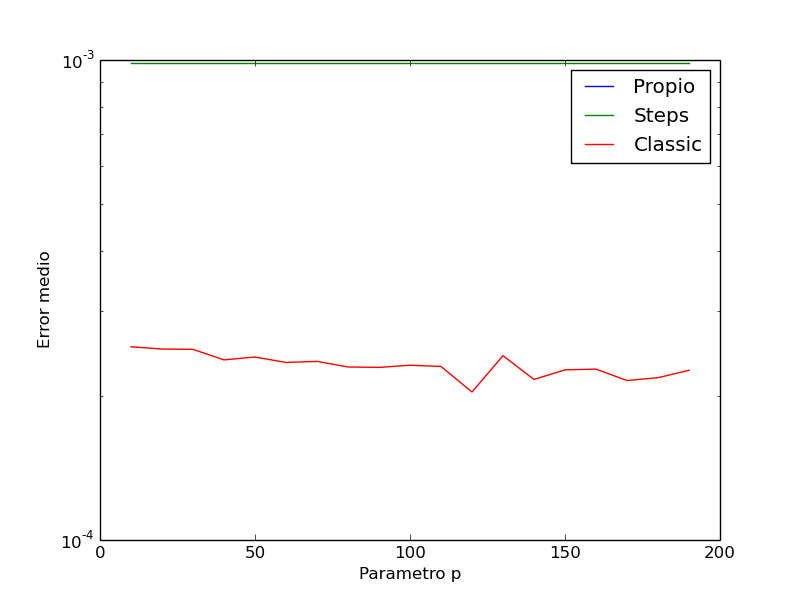
\includegraphics[width=0.45\textwidth]{../source/datasets/img/uniformeEqual}
  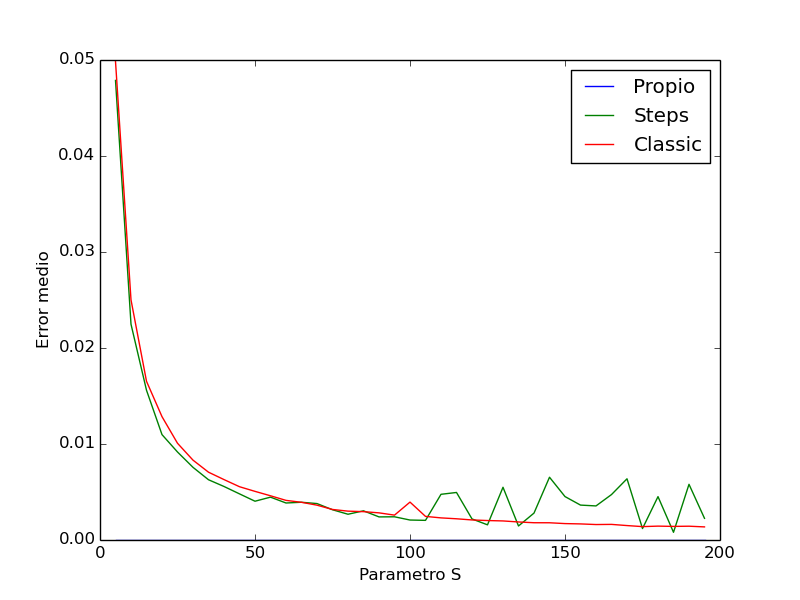
\includegraphics[width=0.45\textwidth]{../source/datasets/img/uniformeGreater}
  \caption{Error medio en función de $S$ para una distribución uniforme, con consultas por igualdad y por mayor respectivamente.}
 \end{figure}
 
 \subsubsection*{Análisis}
Estos datos confirman gran parte del análisis teórico que hicimos en la sección anterior. En primer lugar podemos ver cómo, en el caso de la estimación por igualdad, el parámetro del estimador no modifica de manera alguna la performance. Además, en ese caso la performance de ambos estimadores es muy buena (entre 0.0002 y 0.001), como también habíamos predicho. En el caso de la estimación por mayor confirmamos que en ambos estimadores, a diferencia de la estimación por igualdad, la elección del parámetro cambia drásticamente la performance obtenida, mejorándola al elevar el valor del parámetro.

Un resultado que no estaba contemplado en el análisis teórico es que a partir de cierto valor del parámetro la performance del estimador Distribution Steps oscila erráticamente. Creemos que esto se debe a que llega cierto punto en el que, al tener muchos buckets, comienza a haber valores que aparecen en más de un límite. En esa situación el algoritmo, como ya fue mencionado, caen en el caso en donde intenta minimizar el error en el caso peor caso, obteniendo una performance más pobre en el caso promedio. Intuitivamente podemos decir que pierde precisión al no poder ubicar unívocamente en qué bucket cae el $x_0$ de la consulta.
 
 \subsection{Performance para distribuciones normal}
A continuación mostraremos cómo se comportaron los distintos estimadores en cuanto al error medio obtenido ante la variación del parámetro $S$ de entrada del estimador en una distribución normal. Para cada $S$ fueron realizadas $100$ consultas por igualdad y $100$ consultas por mayor.

La distribución normal utilizada tiene 10000 elementos con $\mu=500$ y $\sigma=100$.


\begin{figure}[h!]  
  \centering
  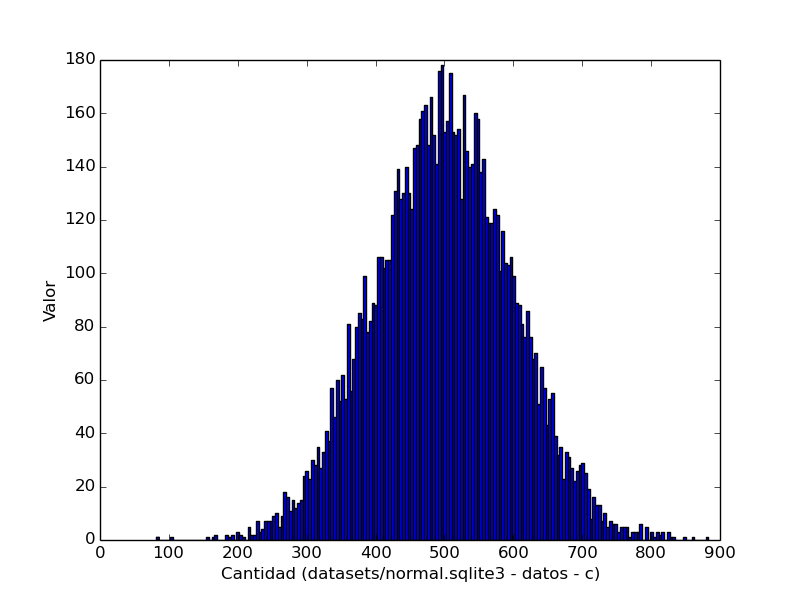
\includegraphics[width=0.45\textwidth]{../source/datasets/img/normal}
  \caption{Distribución utilizada}
 \end{figure}

\begin{figure}[h!]
  \centering
  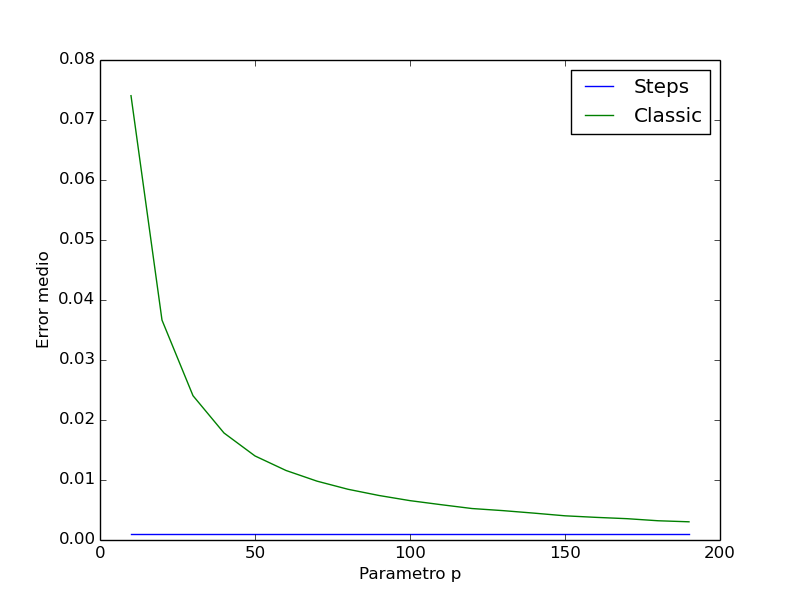
\includegraphics[width=0.45\textwidth]{../source/datasets/img/normalEqual}
  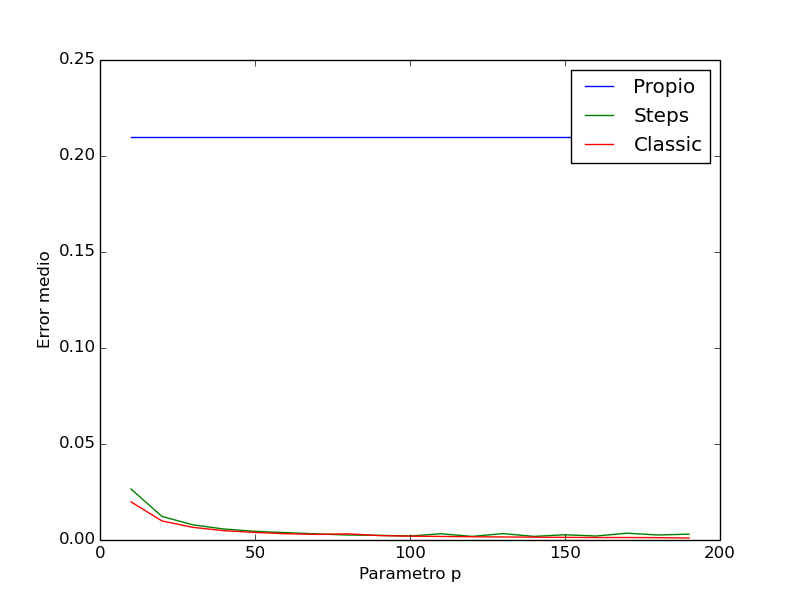
\includegraphics[width=0.45\textwidth]{../source/datasets/img/normalGreater}
  \caption{Error medio en función de $S$ para una distribución normal, con consultas por igualdad y por mayor respectivamente.}
 \end{figure}

 \subsubsection*{Análisis}
Gran parte del análisis es similar al caso uniforme con la excepción de que, como dijimos en el análisis teórico, el estimador clásico debería aumentar la performance al aumentar el parámetro. Esta mejora se aprecia únicamente en los primeros valores del experimento ya que llega rápidamente a una cantidad de buckets que le permite armar un histograma que caracteriza con precisión la distribución de este dataset. En este caso puede verse que el valor se encuentra alrededor de 10 pero en otros datasets este valor podría cambiar, e incluso necesitarse muchos más buckets para llegar al máximo nivel de performance, dependiendo mayormente del $\sigma$ de la distribución.

Observamos nuevamente el comportamiento errático de Distribution Steps para valores grandes de $S$, lo que aumenta la confianza en nuestra hipótesis de que el problema consiste en tener demasiada granularidad en los buckets.

\subsection{Performance para diferentes distribuciones}
En esta sección calculamos la performance de los estimadores en datasets de diferentes distribuciones provistas por la cátedra y análizamos, en cada caso, mediante un test de hipótesis, si alguno de los estimadores es significativamente mejor o si, en términos estadísticos, no existe una diferencia importante de performance. 
El test utilizado es el \textit{Student’s T-Test Apareado} y para realizarlo necesitamos tener dos conjuntos de datos emparentados que representen la información que queremos comparar. En nuestro caso, para comparar el estimador $A$ con el estimador $B$ en cierto dataset, calculamos por un lado la performance de $A$ para estimar valores individuales del dataset y, por otro lado, la performance de $B$ para estimar esos mismos valores. Esto nos da dos listas de datos que están emparentadas por los valores que se estan estimando. Los valores a estimar cubren todo el rango de valores del dataset en intervalos de 10 unidades. Era necesario calcular la performance individual para diferentes valores del dataset y no simplemente tomar la performance como el promedio de todos esos valores ya que el valor promedio no es suficiente información para llevar adelante un test de hipótesis de estas características.

Presentamos a continuación los gráficos de los datasets utilizados:

\begin{figure}[h!]
  \centering
  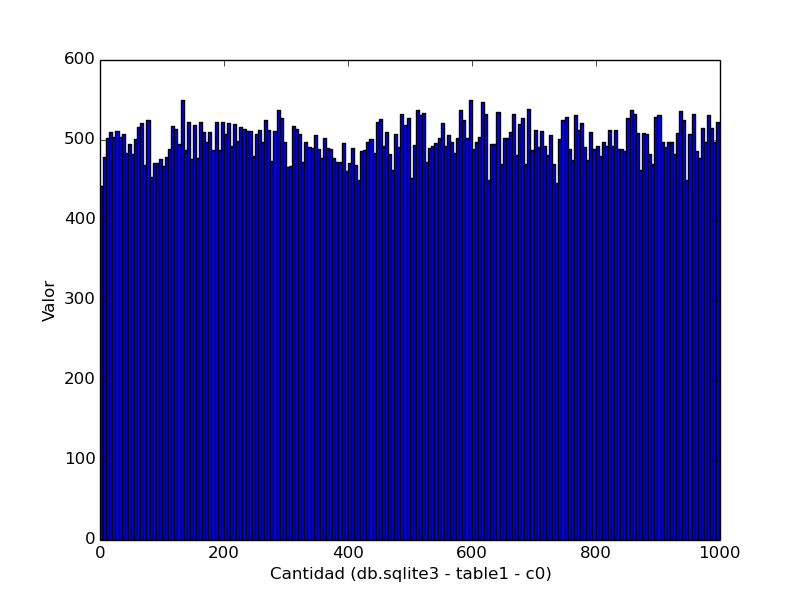
\includegraphics[width=0.45\textwidth]{./../source/datasets/img/c0}
  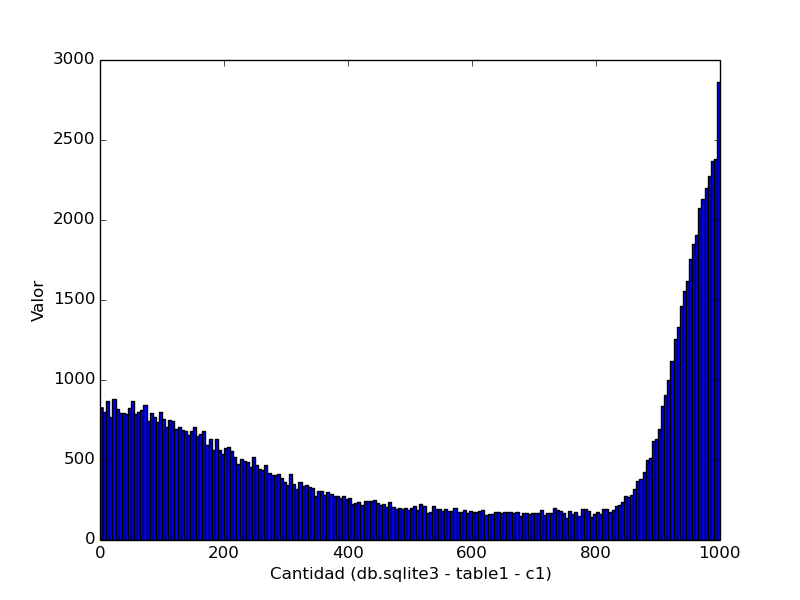
\includegraphics[width=0.45\textwidth]{./../source/datasets/img/c1}
  \caption{Gráficos de los datasets de las columnas c0 y c1}
 \end{figure}
 
 
\begin{figure}[h!]
  \centering
  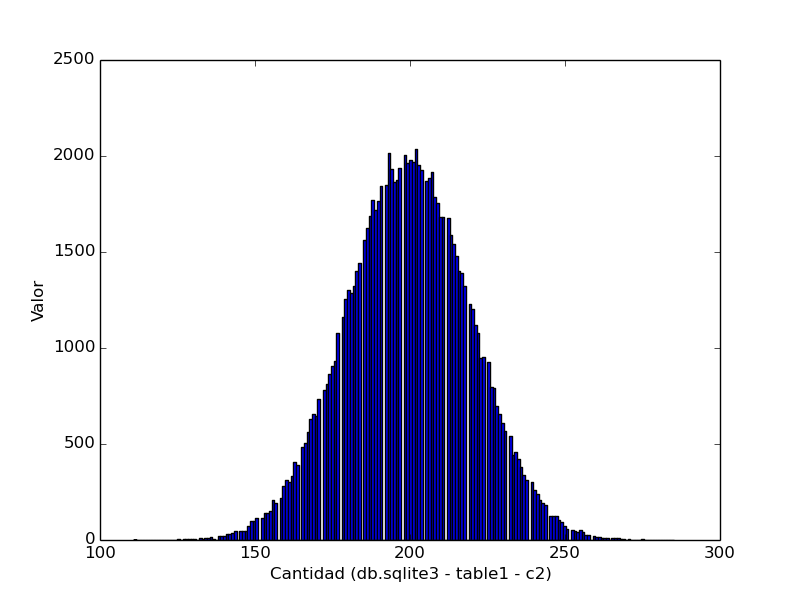
\includegraphics[width=0.45\textwidth]{./../source/datasets/img/c2}
  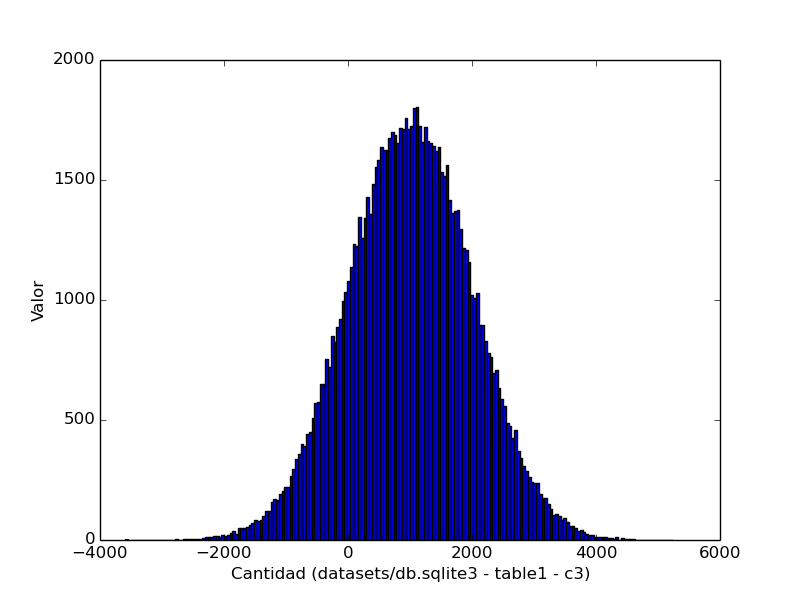
\includegraphics[width=0.45\textwidth]{./../source/datasets/img/c3}
  \caption{Gráficos de los datasets de las columnas c2 y c3}
 \end{figure}
 
\begin{figure}[h!]
  \centering
  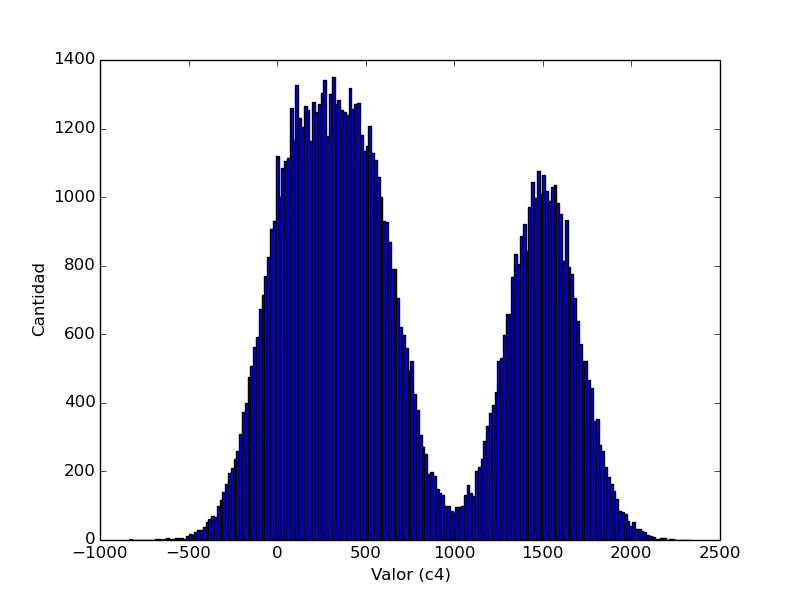
\includegraphics[width=0.45\textwidth]{./../source/datasets/img/c4}
  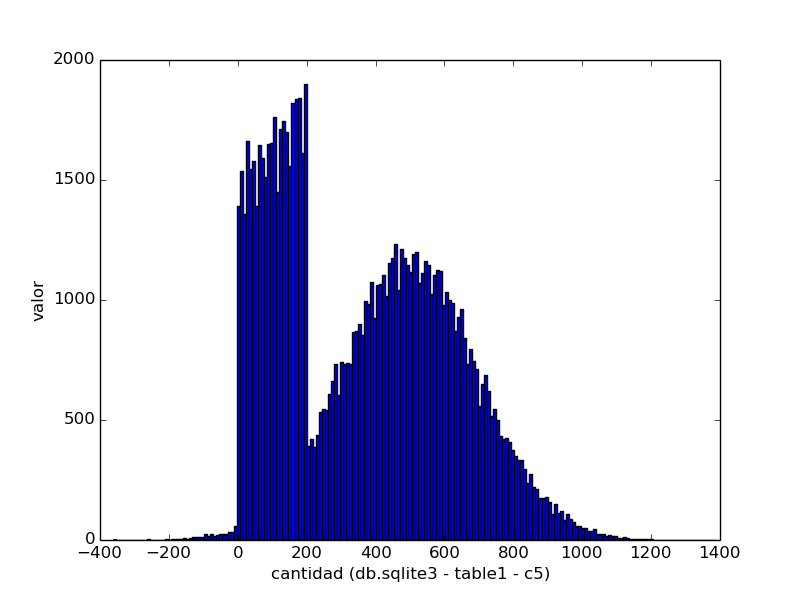
\includegraphics[width=0.45\textwidth]{./../source/datasets/img/c5}
  \caption{Gráficos de los datasets de las columnas c4 y c5}
 \end{figure}
 
 
\begin{figure}[h!]
  \centering
  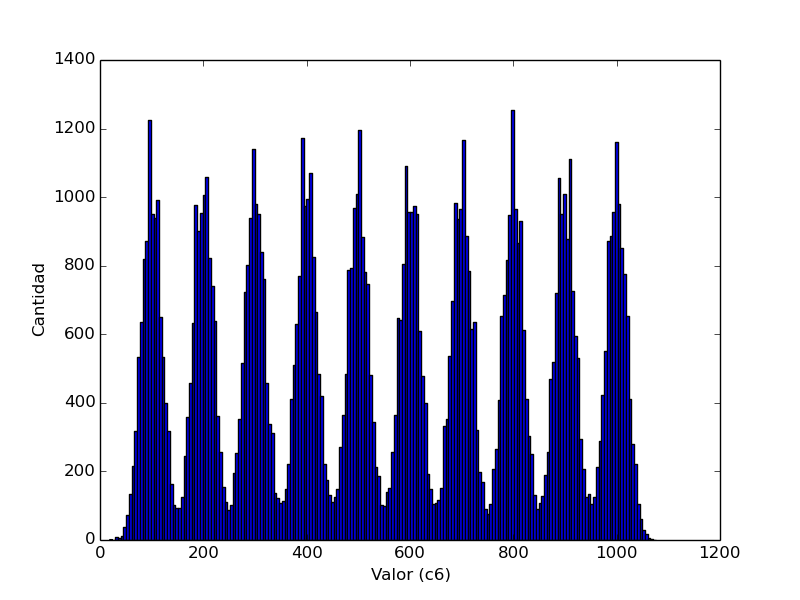
\includegraphics[width=0.45\textwidth]{./../source/datasets/img/c6}
  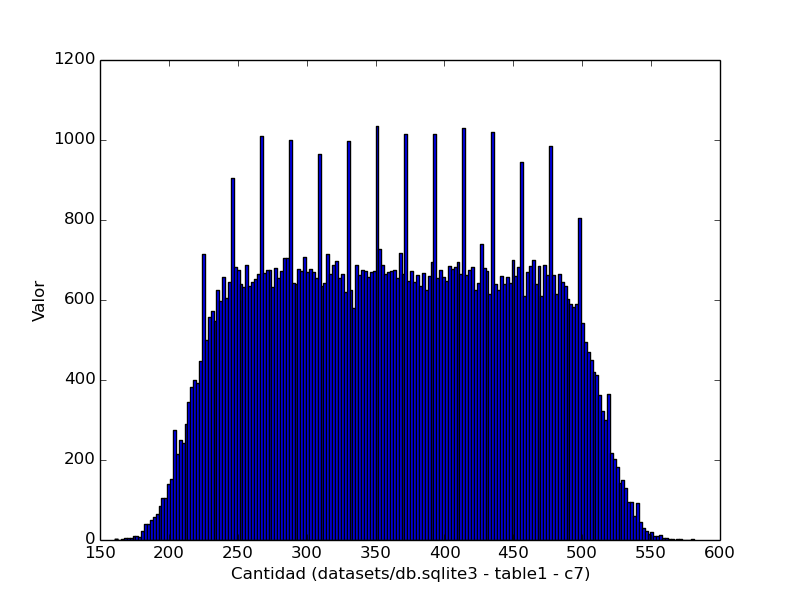
\includegraphics[width=0.45\textwidth]{./../source/datasets/img/c7}
  \caption{Gráficos de los datasets de las columnas c6 y c7}
 \end{figure}
 
 
\begin{figure}[h!]
  \centering
  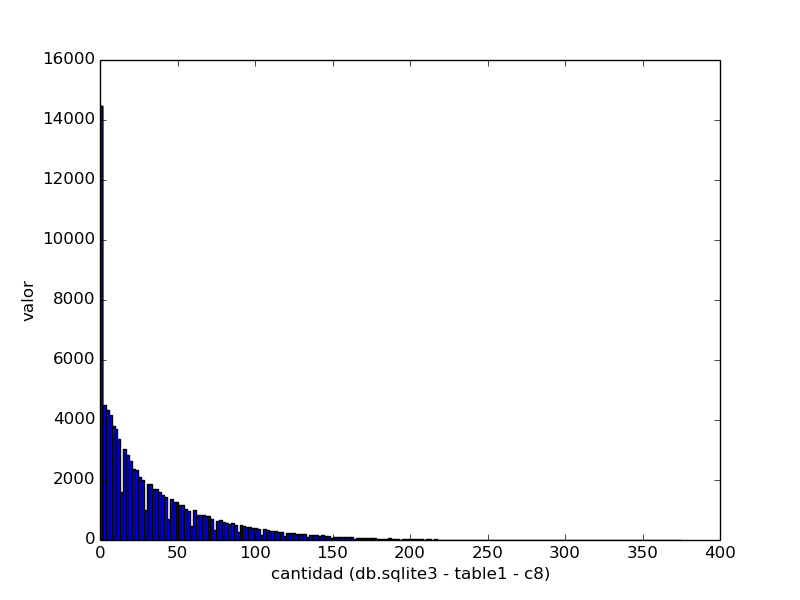
\includegraphics[width=0.45\textwidth]{./../source/datasets/img/c8}
  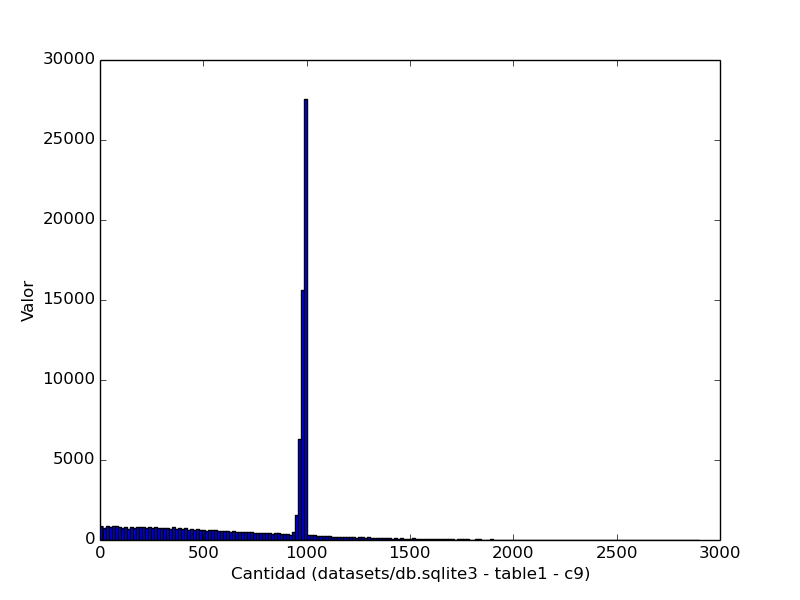
\includegraphics[width=0.45\textwidth]{./../source/datasets/img/c9}
  \caption{Gráficos de los datasets de las columnas c8 y c9}
 \end{figure}
 
\clearpage
Los estimadores que comparamos fueron los dos provistos por el paper y el nuestro, todos con $S=10$, en un enfrentamiento ``triangular''.
El cuadro indica, para una celda en la fila del estimador $X$, en la columna del estimador $Y$, subcolumna de selectividad $W$, en qué datasets de la tabla $X$ ``venció'' a $Y$ para la selectividad $W$, donde ``venció'' quiere decir que tuvo un menor error medio absoluto y que según el \textit{Student’s T-Test Apareado} la diferencia efectivamente fue significativa. La notación $i-j$ en una celda significa todos los valores entre $i$ e $j$, incluyendo ambos. Si un dataset $i$ no aparece ni en la celda $X, Y$ ni en la $Y, X$ para una misma selectividad $W$ hubo un ``empate'' (la diferencia no fue estadísticamente significativa) entre $X$ e $Y$ en ese dataset para esa selectividad.

\begin{table}[h!t]
\centering % centering table
\begin{tabular}{c rrrrrrr} % creating eight columns
\hline\hline %inserting double-line
\ &\multicolumn{2}{c}{Propio}& \multicolumn{2}{c}{Classic}& \multicolumn{2}{c}{Steps} \\ [0.5ex] 
\hline % inserts single-line
 & E & G & E & G & E & G &  \\  
\hline
Propio &X  &X  &0-7, 9 &0-9 &0-9 &0-9 \\ % Entering row contents
\hline
Classic &-  &-  &X &X &1-9 &6 \\
\hline
Steps &-  &- &- &0, 3-5 &X &X  \\[1ex] % [1ex] adds vertical space
\hline % inserts single-line
\end{tabular}
\caption{Comparación entre estimadores.} %title of the table
\label{tab:hresult}
\end{table}

\subsubsection*{Análisis}
Como se puede apreciar en el cuadro \ref{tab:hresult} podemos notar como el estimador creado por nosotros se queda con todas las ``competencias'' entre los estimadores. Esto se debe, como ya mencionamos, a su perfección a nivel de performance. Igualmente vale remarcar que el estimador ``Classic'' logró empatarle (no marcar una diferencia significativa según el \textit{Student’s T-Test Apareado}) en la distribución 8 (una suerte de hipérbola), lo cual significa que anduvo muy bien en ese caso.

\section{Discusión}
Basándonos en nuestro análisis empírico podemos afirmar que los tres estimadores funcionan de manera satisfactoria para distribuciones del tipo uniformes y normales. Esto no debería ser ninguna sorpresa para nosotros, dado que ya fue anticipado por qué debía pasar en la sección 3. Sin embargo, un detalle que no preevimos fue el comportamiento oscilatorio de las comparaciones por mayor del estimador \textbf{Steps} para valores grandes de $S$. Como ya comentamos, este fenómeno se debe a que al agrandarse la cantidad de buckets aumenta significativamente la cantidad de elementos que coinciden con dos o más límites entre buckets (ver sección 2.2, 4.4.1 y 4.4.2).

Analizemos primero las diferencias entre los dos estimadores propuestos por la cátedra.

Mirando el cuadro \ref{tab:hresult} podemos notar que el estimador \textbf{Classic} suele comportarse muy bien en \textbf{todas} las columnas de la base otorgada por la cátedra a la hora de consultar por igualdad. Basándonos en esto, podemos decir que si sabemos de antemano que la mayor parte de las consultas hechas al motor de optimizaciones de la base serán por igualdad, no dudaríamos en elegir \textbf{Classic} sobre \textbf{Steps}.

No ocurre lo mismo cuando la consulta es de selectividad por mayor, como ya fue adelantado por nosotros en diversos puntos. De hecho se ``invierten'' los papeles y quien logra mejores resultados es el estimador \textbf{Steps}. Análogamente entonces, de saber que la mayor parte de consultas será por mayor (o por desigualdades en general) nos inclinaríamos por utilizar \textbf{Steps} (aunque con un valor de $S$ no muy grande).

Igualmente, dado que existen muchos empates en el caso de selectividad por mayor, creemos que la ventaja general la sigue teniendo \textbf{Classic}. Con lo cual para el caso general, si tuviésemos que elegir uno de los dos para tomarlo como estimador sin saber de antemano qué tipo de consultas será la más frecuente, elegiríamos \textbf{Classic}.

Dicho esto, y considerando como ya se mencionó que nuestro estimador es estrictamente mejor que \textbf{Classic} en el caso general y mucho mejor en algunos casos particulares, parecería un buen candidato a ganador para una distribución desconocida de antemano. Sin embargo, presenta problemas similares a \textbf{Classic} a la hora de calcular por mayor en ciertas distribuciones con mucha concentración de datos, con lo cual no podemos declararlo correcto para todos los casos. Además, su consumo de memoria es el triple, pues agrega al histograma dos estructuras extra también de tamaño $S$.

Es por esto que entendemos que difícilmente haya un estimador que funcione de modo correcto en todos los casos. Por lo menos para todos los que pudimos analizar encontramos casos en donde podría funcionar mal (ver sección 3.4).

Como agregado, podemos mencionar que las tres implementaciones tardan tiempo en inicializarse, pero la idea es que cuando alguien realice una consulta a la base demoren muy poco tiempo en devolver una respuesta que se considere correcta. Es necesario que sea rápido dada que se hacen muchas consultas SQL por unidad de tiempo en un servidor. En cambio la creación de cero de un estimador no es tan frecuente, y se pueden aprovechar las noches (o los momentos de menos tráfico) para actualizarlo. 

\section{Conclusiones}
A lo largo del TP comprendimos que el problema de estimar la selectividad en una columna de una tabla no es trivial, sino que esconde todo un mundo de matemáticas, decisiones algoritmicas, de velocidad, de consumo de memoria de mayor o menor precisión. Implementamos diversos estimadores recomendados y diseñamos uno propio que funcionó perfectamente pero con gran costo espacial y temporal en casos generales.

Analizamos la performance de los estimadores con diferentes distribuciones de datos, y concluimos que no hay un claro ganador para todas las distribuciones, sino que cada uno presenta ventajas y desventajas y que hace falta conocer el dominio en el que se van a utilizar para sacarles todo el jugo posible.

Descubrimos también que el estimador ``perfecto'' trae asociado siempre un gran costo, ya sea en velocidad o en memoria (o ambas).

La mayor parte de nuestras predicciones teóricas se verificaron en la práctica, pero encontramos una situación curiosa según la cual aumentar en exceso un parámetro que pensábamos estaba directamente asociado con la ``precisión'' terminaba repercutiendo negativamente en la performance del estimador, dada su implementación algorítmica.

Como conclusión general de nuestras comparaciones, sostenemos que nuestro estimador se comporta bien en el caso general si se pueden aceptar sus problemas de memoria y performance en ciertos casos. Si esto no es posible, priorizaríamos la elección del Histograma Clásico en el caso general, y solo eligiríamos el Steps si sabemos de antemano que las consultas presentarán mayormente desigualdades.

\end{document}